\section{The Simple Series archetype}
\begin{frame}
  \frametitle{The simple serie archetype}

  \begin{definition}[Simple serie archetype]
    A series of $n$ neurons $N_1, ..., N_n$, where $N_i$ receives the signal form $N_{i-1}$ and emits its signal to $N_{i+1}$.
  \end{definition}

  \mysep{}

  There exists $2$ main implementations of this archetype:
  \begin{itemize}
    \item the $n$-delayer
    \item the $n$-delayer/filter
  \end{itemize}

\end{frame}

\begin{frame}[fragile]
  \frametitle{The $n$-delayer}

  Given a signal $\mathcal{S}$, $\mathcal{S}$ is transmitted with a delay of $n$ time units.

  \mysep{}

  Implementation:

  \begin{figure}
    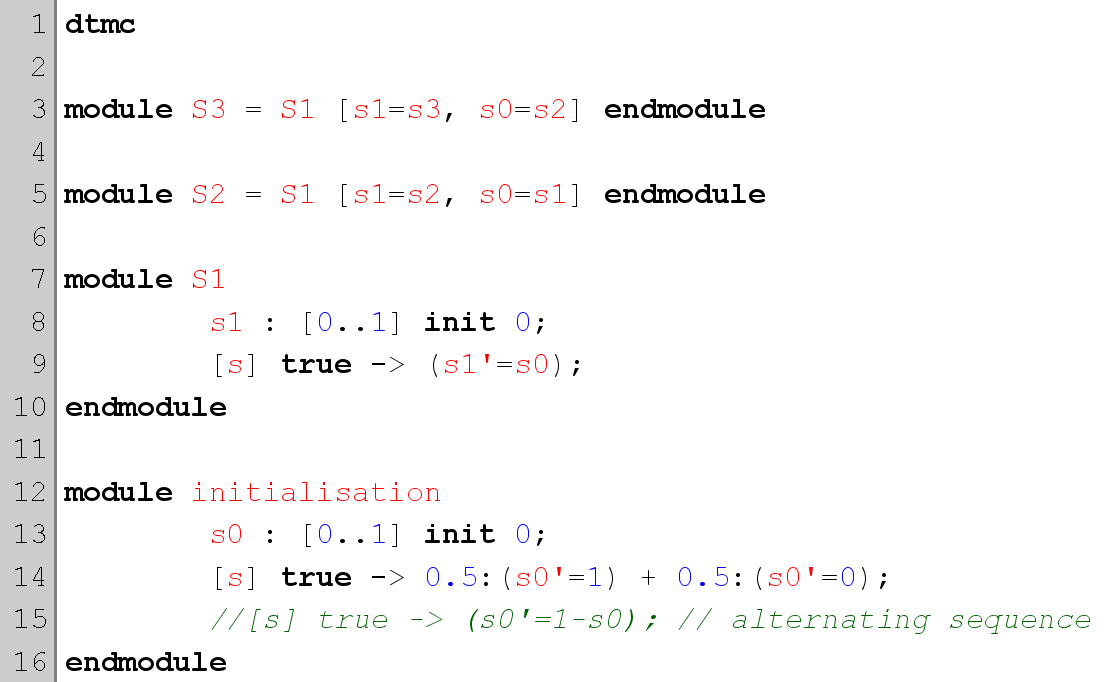
\includegraphics[width=0.7\textwidth]{pic/simple_serie1_code.png}
  \end{figure}

\end{frame}

\begin{frame}
  \frametitle{A plot of a $n$-delayer}

  \begin{figure}
    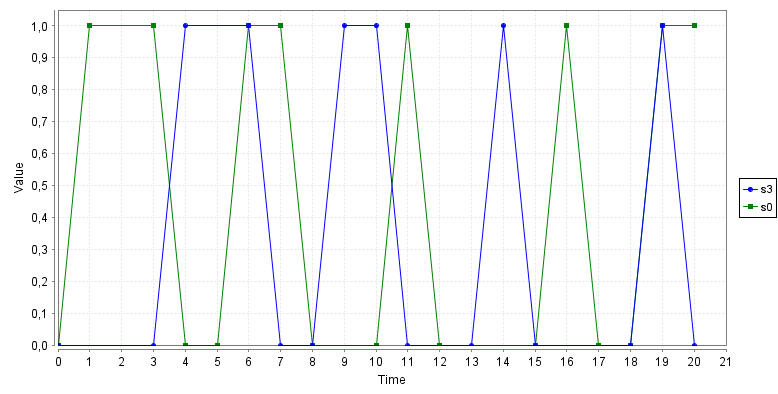
\includegraphics[width=0.8\textwidth]{pic/simple_serie1_plot.png}
  \end{figure}

  \mysep{}

  An interesting property:
  \begin{itemize}
    \item $P = [G (s_0 = 1 \Leftrightarrow X^3 (s_3=1))] ? $ \uncover<2->{$1.0$}
  \end{itemize}

\end{frame}

\begin{frame}
  \frametitle{The $n$-delayer/filter}

  Let's introduce the leak factor and the potential membrane:\\ An example of \textbf{code corrector}.

  \begin{figure}
    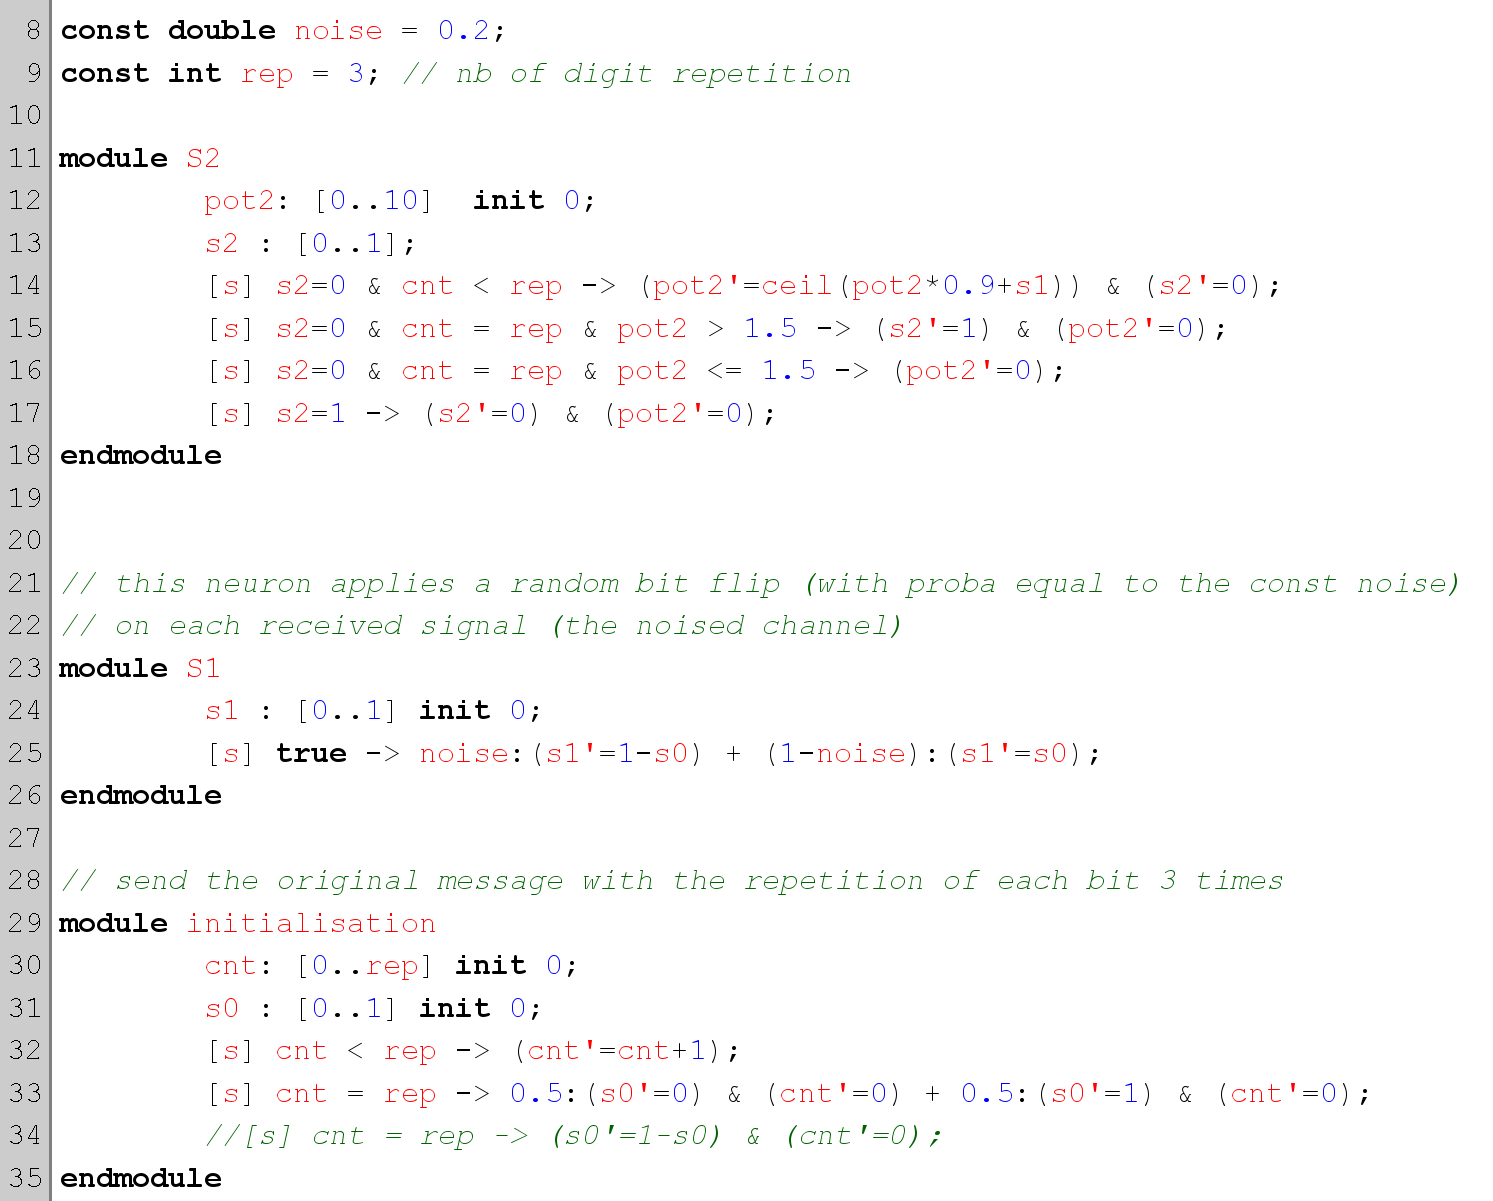
\includegraphics[width=0.62\textwidth]{pic/simple_serie_corr_code.png}
  \end{figure}

\end{frame}

\begin{frame}
  \frametitle{A plot of a $n$-delayer/filter}

  % \begin{figure}
  %   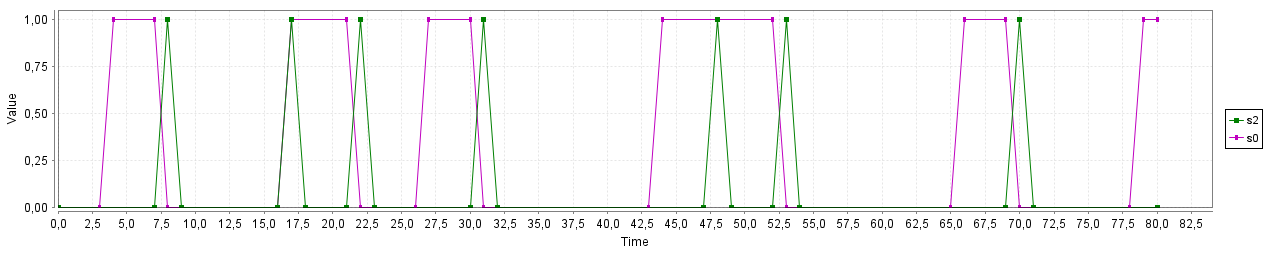
\includegraphics[width=0.9\textwidth]{pic/simple_serie_corr_plot.png}
  % \end{figure}

  % \begin{figure}
  %   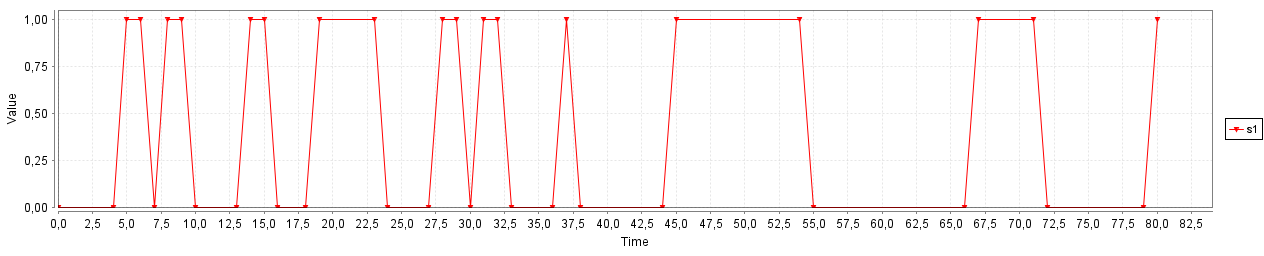
\includegraphics[width=0.9\textwidth]{pic/simple_serie_corr_plot_s1.png}
  % \end{figure}

  \begin{figure}
    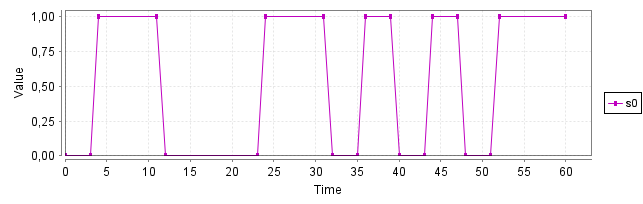
\includegraphics[width=0.54\textwidth]{../my_models/1serieDelFil_Corrector/plot_S0.png}
  \end{figure}

  \begin{figure}
    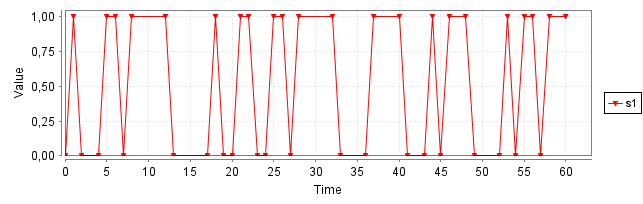
\includegraphics[width=0.54\textwidth]{../my_models/1serieDelFil_Corrector/plot_S1.png}
  \end{figure}

  \begin{figure}
    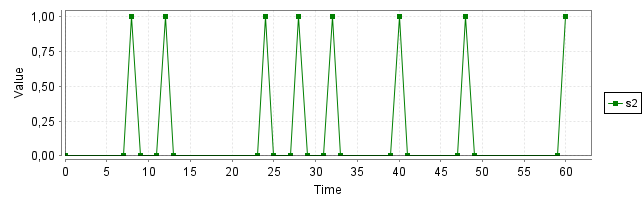
\includegraphics[width=0.54\textwidth]{../my_models/1serieDelFil_Corrector/plot_S2.png}
  \end{figure}

\end{frame}

\begin{frame}
  \frametitle{Test certainty of model by noise}
  \begin{align*}
    P \stackrel{?}{=} &
    % \begin{cases}
    % (X^4 ((s_0=1) \Leftrightarrow X^5 (s_2=1))) & \text{if } noise > 0.5 \\
    (X^4 ((s_0=1) \Leftrightarrow X^4 (s_2=1)))
    % \end{cases}
  \end{align*}



  \uncover<2->{
    % \begin{columns}
    %   \begin{column}{1\textwidth}
    \begin{table}[]
      \begin{tabular}{cc}
        noise                & proba                \\ \hline
        $0.00$               & $1.00$               \\
        \uncover<3->{$0.10$} & \uncover<3->{$0.90$} \\
        \uncover<4->{$0.50$} & \uncover<4->{$0.50$} \\
        \uncover<5->{$0.90$} & \uncover<5->{$0.10$} \\
        \uncover<6->{$1.00$} & \uncover<6->{$0.00$}
      \end{tabular}
    \end{table}
    % \end{column}
    % \begin{column}{0.55\textwidth}  %%<--- here
    %   \begin{remark}
    %     If the $noise$ is bigger than $0.5$, we have to look at the fifth time-unit: one time-unit is consumed by the $reset$ action.
    %   \end{remark}
    % \end{column}
    % \end{columns}
  }

\end{frame}